\documentclass[a4paper,12pt]{report}            % [forma A4, taille police] {Type}
\usepackage[utf8]{inputenc}                
\usepackage[T1]{fontenc}                        % Codage des fontes TeX
\usepackage[francais]{babel}
\usepackage{graphicx}
\usepackage{wrapfig}
\usepackage{fancyhdr}
\usepackage{xcolor}
\usepackage{hyperref}
\usepackage{listings}
\usepackage{fullpage}
\usepackage{eso-pic}
\usepackage{titlesec}
\titleformat{\chapter}[hang]{\bf\huge}{\thechapter}{2pc}{}
\lstset {numbers=left ,stepnumber=1,firstnumber=0,numberfirstline=true}
\hypersetup{
    bookmarks=true,         % show bookmarks bar?
    unicode=false,          % non-Latin characters in Acrobat’s bookmarks
    pdftoolbar=true,        % show Acrobat’s toolbar?
    pdfmenubar=true,        % show Acrobat’s menu?
    pdffitwindow=false,     % window fit to page when opened
    pdfstartview={FitH},    % fits the width of the page to the window
    pdftitle={My title},    % title
    pdfauthor={Author},     % author
    pdfsubject={Subject},   % subject of the document
    pdfcreator={Creator},   % creator of the document
    pdfproducer={Producer}, % producer of the document
    pdfkeywords={keyword1, key2, key3}, % list of keywords
    pdfnewwindow=true,      % links in new PDF window
    colorlinks=true,       % false: boxed links; true: colored links
    linkcolor=black,          % color of internal links (change box color with linkbordercolor)
    citecolor=green,        % color of links to bibliography
    filecolor=magenta,      % color of file links
    urlcolor=blue           % color of external links
}

\author{Samuel HUET \& Thomas COUTANT}
\title{\huge{Le Mixer}}

\begin{document}
\maketitle
\renewcommand{\contentsname}{SOMMAIRE} % Dans le corps du document,avant la commande \tableofcontents.
\tableofcontents

\chapter{Le mélangeur à diode}
\addcontentsline{toc}{chapter}{Le mélangeur à diode}

\section{Principe de fonctionnement}
    Un mélangeur permet de transposer un signal radio (RF) par soustraction ou addition avec
une autre fréquence venant d'un oscillateur local (OL). Nous obtenons donc en sortie des
signaux (FI) aux fréquences $FI = |OL - RF|$ ou $FI = |OL + RF|$\\
    Le mélangeur à diodes utilise l'équation liant tension/courant non linéaire
des diodes afin de réalise le mélange. Il est consitué de 4 diodes et de deux transformateurs.
Bien que le mélangeur à diode génère moins moins de signaux indésirables que certains autres montages,
il s'agit d'une structure passive, qui assure une perte d'un moins 6dB sur sa sortie.\\
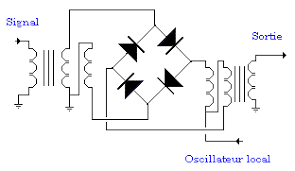
\includegraphics[scale = 1]{/home/cocasticox/Documents/LaTeX/Radio/TP1/pic/schema_mixer.png}\\
    La non linéarité des diodes implique inévitablement des signaux parasites sur la sortie,
pouvant s'écrire : $Vs = a + b(Ve) + c(Ve)^{2} + d(Ve)^{3} ...$\\
    Pour des signaux d'entrée dont l'excursion est faible, la  droite de charge de la diode peut 
être aproximé à une droite, mais les signaux dont l'excursion est plus large implique des signaux parasites.\\
    Voici le schema du melangeur. Nous pouvons y voir les fréquences d'entré $F_{RF}$, $F_{OL}$ ainsi que la
fréquence de sortie $F_{IF}$ expliqués plus haut. Celui que nous allons utiliser pour ce TP est le ZFM-2 de Mini Circuits.\\
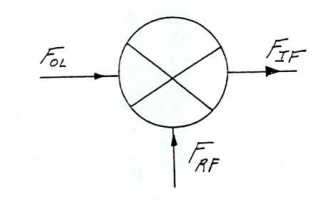
\includegraphics[scale = 0.4]{/home/cocasticox/Documents/LaTeX/Radio/TP1/pic/mixer_logo.png}\\



\end{document}

